\documentclass[a4paper,oneside,12pt]{report}
\setlength\textwidth{155mm}
\setlength\textheight{247mm}
\setlength\topmargin{-10mm}
\setlength\headheight{0mm}
\setlength\oddsidemargin{05mm}
\setlength\evensidemargin{05mm}
\let\openright=\clearpage


%% Vytváříme PDF/A-2u
\usepackage[a-2u]{pdfx}

%% Přepneme na českou sazbu a fonty Latin Modern
\usepackage[czech]{babel}
\usepackage{lmodern}
\usepackage[T1]{fontenc}
\usepackage{textcomp}

%% Použité kódování znaků: obvykle latin2, cp1250 nebo utf8:
\usepackage[utf8]{inputenc}

%%% Další užitečné balíčky (jsou součástí běžnýsrov.stribucí LaTeXu)
\usepackage{amsmath}        % rozšíření pro sazbu matematiky
\usepackage{amsfonts}       % matematické fonty
\usepackage{amsthm}         % sazba vět, definic apod.
\usepackage{bbding}         % balíček s nejrůznějšími symboly
			   										% (čtverečky, hvězdičky, tužtičky, nůžtičky, ...)
\usepackage{bm}             % tučné symboly (příkaz \bm)
\usepackage{graphicx}       % vkládání obrázků
\usepackage{fancyhdr}				% možnost slylizovat záhlaví
\usepackage{fancyvrb}       % vylepšené prostředí pro strojové písmo
% \usepackage{indentfirst}    % zavede odsazení 1. odstavce kapitoly
\usepackage[nottoc]{tocbibind} % zajistí přidání seznamu literatury,
\usepackage{icomma}         % inteligetní čárka v matematickém módu
\usepackage{dcolumn}        % lepší zarovnání sloupců v tabulkách
\usepackage{booktabs}       % lepší vodorovné linky v tabulkách
\usepackage{paralist}       % lepší enumerate a itemize
\usepackage{caption}				%	popisky
\usepackage{dirtree}				% strom souborů
\usepackage{listings}				% vkládání kódu
\usepackage[bottom]{footmisc}  % poznámky pod čarou vespod
\usepackage{bibentry}
\usepackage{xurl}						% umožní url zalomit všude
\nobibliography*
\usepackage{float}

\usepackage{color}
\usepackage{forest}					% na rodokmeny
\usepackage{natbib}
\usepackage{enumitem}

%\setbibentrystyle{author}

\newlist{algEnumerate}{enumerate}{10}
\setlist[algEnumerate]{label*=\arabic*.}
\setlist*[algEnumerate]{nosep} 
\definecolor{pblue}{rgb}{0.13,0.13,1}
\definecolor{pgreen}{rgb}{0,0.5,0}
\definecolor{pred}{rgb}{0.9,0,0}
\definecolor{pgrey}{rgb}{0.46,0.45,0.48}
\definecolor{apiblue}{HTML}{000000}
\definecolor{apigreen}{HTML}{000000}
\definecolor{apicyan}{HTML}{000000} % vím, že cyan je jiná barva % vím, že cyan je jiná barva
\definecolor{apired}{HTML}{000000}
\definecolor{apiyellow}{HTML}{000000}
% \definecolor{apiblue}{HTML}{61AFFE}
% \definecolor{apigreen}{HTML}{49CC90}
% \definecolor{apicyan}{HTML}{50E3C2} % vím, že cyan je jiná barva % vím, že cyan je jiná barva
% \definecolor{apired}{HTML}{F93E3E}
% \definecolor{apiyellow}{HTML}{FCA130}
\renewcommand{\baselinestretch}{1.5}
%%% Údaje o práci

\def\NazevSkoly{Gymnázium, Praha 6, Arabská 14}
% Název oboru včetně počátečního 'Obor'.
\def\NazevOboru{Programování}

% Název práce v jazyce práce (přesně podle zadání)
\def\NazevPrace{Sudoku se vším všudy}

% Název práce v angličtině
\def\NazevPraceEN{Sudoku with everything in it}

% Název práce v němčině
\def\NazevPraceDE{Sudoku mit allem, was dazugehört}

% Jméno autra
\def\AutorPrace{Vladimír Vávra, 4.E}

% Rok odevzdání
\def\RokOdevzdani{2022}
% Měsíc odevzdání
\def\MesicOdevzdani{Únor}

% Vedoucí práce: Jméno a příjmení s~tituly
\def\Vedouci{Ing. Daniel Kahoun}

% Nepovinné poděkování (vedoucímu práce, konzultantovi, tomu, kdo
% zapůjčil software, literaturu apod.)
\def\Podekovani{%
Rád bych zde poděkoval Kryštofu Havránkovi za zapůjčení LaTeX vzoru pro dokumentaci a prezentaci.
}

% Abstrakt (doporučený rozsah cca 80-200 slov; nejedná se o zadání práce)
\def\Abstrakt{%
Vytvořte webovou aplikaci, jejímž primárním účelem je hraní sudoku v klasické podobě i možných variantách lišících se typem hracího pole i počtem hráčů. Aplikace dokáže sudoku vyřešit a vygenerovat zadání, u základní varianty na základě obtížnosti. 
}

\def\AbstraktEN{%
Create a web application whose primary purpose is to play sudoku in its classic form and possible variations differing in the type of playing field and the number of players. The application can solve the sudoku and generate the assignment, for the basic variant based on difficulty. 
}
\def\AbstraktDE{%
Erstellen Sie eine Webanwendung, deren Hauptzweck darin besteht, Sudoku in seiner klassischen Form und möglichen Varianten zu spielen, die sich in der Art des Spielfelds und der Anzahl der Spieler unterscheiden. Die Anwendung kann das Sudoku lösen und die Aufgabe für die Grundvariante nach Schwierigkeitsgrad erstellen. 
}
% 3 až 5 klíčových slov (doporučeno), každé uzavřeno ve složených závorkách
\def\KlicovaSlova{%
	{sudoku}, {javascript}, {nodejs}, {react js}
}
\def\KlicovaSlovaEN{%
   {sudoku}, {javascript}, {nodejs}, {react js}
}

\def\KlicovaSlovaDE{%
   {sudoku}, {javascript}, {nodejs}, {react js}
}

%% Balíček hyperref, kterým jdou vyrábět klikací odkazy v PDF,
%% ale hlavně ho používáme k uložení metadat do PDF (včetně obsahu).
%% Většinu nastavítek přednastaví balíček pdfx.
\hypersetup{unicode}
\hypersetup{breaklinks=true}

%% Definice různých užitečných maker (viz popis uvnitř souboru)
%%% Tento soubor obsahuje definice různých užitečných maker a prostředí %%%
%%% Další makra připisujte sem, ať nepřekáží v ostatních souborech.     %%%

%%% Drobné úpravy stylu

% Tato makra přesvědčují mírně ošklivým trikem LaTeX, aby hlavičky kapitol
% sázel příčetněji a nevynechával nad nimi spoustu místa. Směle ignorujte.
\makeatletter
\def\@makechapterhead#1{
  {\parindent \z@ \raggedright \normalfont
   \Huge\bfseries \thechapter. #1
   \par\nobreak
   \vskip 20\p@
}}
\def\@makeschapterhead#1{
  {\parindent \z@ \raggedright \normalfont
   \Huge\bfseries #1
   \par\nobreak
   \vskip 20\p@
}}
\makeatother

% Toto makro definuje kapitolu, která není očíslovaná, ale je uvedena v obsahu.
\def\chapwithtoc#1{
\chapter*{#1}
\addcontentsline{toc}{chapter}{#1}
}

% Trochu volnější nastavení dělení slov, než je default.
\lefthyphenmin=2
\righthyphenmin=2

% Zapne černé "slimáky" na koncích řádků, které přetekly, abychom si
% jich lépe všimli.
\overfullrule=1mm

%%% Makra pro definice, věty, tvrzení, příklady, ... (vyžaduje baliček amsthm)

\theoremstyle{plain}
\newtheorem{veta}{Věta}
\newtheorem{lemma}[veta]{Lemma}
\newtheorem{tvrz}[veta]{Tvrzení}

\theoremstyle{plain}
\newtheorem{definice}{Definice}

\theoremstyle{remark}
\newtheorem*{dusl}{Důsledek}
\newtheorem*{pozn}{Poznámka}
\newtheorem*{prikl}{Příklad}

%%% Prostředí pro důkazy

\newenvironment{dukaz}{
  \par\medskip\noindent
  \textit{Důkaz}.
}{
\newline
\rightline{$\square$}  % nebo \SquareCastShadowBottomRight z balíčku bbding
}

%%% Prostředí pro sazbu kódu, případně vstupu/výstupu počítačových
%%% programů. (Vyžaduje balíček fancyvrb -- fancy verbatim.)

\DefineVerbatimEnvironment{code}{Verbatim}{fontsize=\small, frame=single}

%%% Prostor reálných, resp. přirozených čísel
\newcommand{\R}{\mathbb{R}}
\newcommand{\N}{\mathbb{N}}

%%% Užitečné operátory pro statistiku a pravděpodobnost
\DeclareMathOperator{\pr}{\textsf{P}}
\DeclareMathOperator{\E}{\textsf{E}\,}
\DeclareMathOperator{\var}{\textrm{var}}
\DeclareMathOperator{\sd}{\textrm{sd}}

%%% Příkaz pro transpozici vektoru/matice
\newcommand{\T}[1]{#1^\top}

%%% Vychytávky pro matematiku
\newcommand{\goto}{\rightarrow}
\newcommand{\gotop}{\stackrel{P}{\longrightarrow}}
\newcommand{\maon}[1]{o(n^{#1})}
\newcommand{\abs}[1]{\left|{#1}\right|}
\newcommand{\dint}{\int_0^\tau\!\!\int_0^\tau}
\newcommand{\isqr}[1]{\frac{1}{\sqrt{#1}}}

%%% Vychytávky pro tabulky
\newcommand{\pulrad}[1]{\raisebox{1.5ex}[0pt]{#1}}
\newcommand{\mc}[1]{\multicolumn{1}{c}{#1}}


%% Titulní strana a různé povinné informační strany
\fancypagestyle{plain}{
\fancyhf{}
\renewcommand{\headrulewidth}{0.4pt}
\renewcommand{\footrulewidth}{0.4pt}
\fancyhead[C]{}
\fancyhead[L]{Ročníková práce -- \NazevSkoly}
\fancyhead[R]{Sudoku se vším všudy}
\fancyfoot[L]{Vypracovali: \AutorPrace}
\fancyfoot[C]{}
\fancyfoot[R]{\thepage}
}



\begin{document}

%%% Titulní strana práce

\pagestyle{empty}
\hypersetup{pageanchor=false}

\begin{center}

{\LARGE\bfseries\NazevSkoly}

\vspace{-18mm}
\vfill

{\LARGE\NazevOboru}

\vfill

\centerline{\mbox{
\includegraphics[height=4cm]{../img/logo.png}}}

\vspace{-8mm}
\vfill

{\bf\Large MATURITNÍ PRÁCE}

\vfill


\vspace{15mm}

{\LARGE\bfseries\NazevPrace}


\vfill


Vypracoval: \hfill \AutorPrace

Vedoucí práce: \hfill \Vedouci

\vspace{15mm}
\MesicOdevzdani \ \RokOdevzdani

\end{center}



\newpage
\hypersetup{pageanchor=true}
\pagestyle{plain}
\pagenumbering{gobble}


\openright


\vspace*{\fill}


\noindent
Prohlašuji, že jsem jediným autorem tohoto projektu, všechny citace jsou
řádně označené a všechna použitá literatura a další zdroje jsou v práci uvedené.
Tímto dle zákona 121/2000 Sb. (tzv. Autorský zákon) ve znění pozdějších předpisů uděluji
bezúplatně škole Gymnázium, Praha 6, Arabská 14 oprávnění k výkonu práva na rozmnožování díla
(§ 13) a práva na sdělování díla veřejnosti (§ 18) na dobu časově neomezenou a bez omezení
územního rozsahu.


\vspace{1cm}

\noindent
V ........ dne ............
\hspace{4cm}
Podpis autora


\newpage
%
% %%% Poděkování
%
\openright

\noindent
\Podekovani



% \newpage


\openright

\vbox to 0.20\vsize{
\setlength\parindent{0mm}
\setlength\parskip{5mm}

Název práce:
\NazevPrace

Autoři:
\AutorPrace

% Vedoucí práce:
% \Vedouci, \KatedraVedouciho

Abstrakt:
\Abstrakt

Klíčová slova:
\KlicovaSlova

% Opakování v angličtině.

Title:
\NazevPraceEN

Authors:
\AutorPrace

Abstract:
\AbstraktEN

Key words:
\KlicovaSlovaEN


% Opakování v němčině.

Titlel:
\NazevPraceDE

Autoren:
\AutorPrace

Abstrakt:
\AbstraktDE

Schlüsselwörter:
\KlicovaSlovaDE

\vss}

\newpage

\openright



\tableofcontents


\newpage

\chapter*{Úvod}
\pagenumbering{gobble}
\addcontentsline{toc}{chapter}{Úvod}

Zadáním projektu bylo vytvořit webovou aplikaci, jejímž primárním účelem je hraní sudoku v klasické podobě i možných variantách. Aplikace dokáže sudoku vyřešit a vygenerovat zadání. Kromě klasického sudoku dokáže také vygenerovat zadání na základě obtížnosti pro všechny typy, u kterých je aktuálně generování podporováno, čímž se práce rozšířila.

Kromě tohoto také aplikace poskytuje základní funkce vnitřní ekonomiky, jako je možnost různých typů přihlášení a nakupování vylepšení za interní měnu.

Co se použitých technologií píše, frontend byl napsán v knihovně ReactJS, backend v NodeJS s frameworkem Express a jako databáze byla použita MongoDB. V každé z těchto částí je využito mnoha knihoven, které jsou specifikovány v souborech \texttt{package.json}, jenž nacházejí přímo ve zdrojovém kódu.

\pagenumbering{arabic}
\setcounter{page}{1}

\chapter{Sudoku}
Tuto hru vymyslel Howard Garns v roce 1979 a publikoval ji v pod názvem „Number Place“. Své velké obliby se dočkala v Japonsku, odkud se později vrátila zpět pod názvem „sudoku“. Ve světě je sudoku vydáváno v mnoha periodikách. U nás jsou to např. Lidové noviny, MF Dnes, Právo, Deník či Metro.

Cílem hry v základní podobě je doplnit chybějící cifry 1 až 9 v zadané, zčásti vyplněné čtvercové tabulce s 9 × 9 poli. V tabulce jsou zvýrazněny sekce vymezující 9 čtverců (3 × 3).

K předem vyplněným číslicím je třeba doplnit další číslice tak, aby platilo, že v každém řádku, v každém sloupci a v každém z devíti dílčích čtverců jsou použity vždy všechny číslice jedna až devět, každá právě jednou.

Aritmetická hodnota číslic pro řešení nemá význam, jde pouze o výběr logické řady devíti znaků (v zásadě je možné hrát sudoku i např. s písmeny A–I nebo jakoukoli jinou skupinou devíti symbolů).

Všech různých možností, jak může být hrací pole 9 × 9 podle těchto kritérií sestaveno, je 6 670 903 752 021 072 936 960, tj. přibližně 6,67×1021 (6,67 triliard). Pro zvětšující se čtverce je to úloha NP-úplná.
\footnote{\bibentry{Sudoku}}

\section{Typy her}
Tato aplikace dovoluje uživateli hrát různé varianty sudoku lišící se pravidly pro doplňování čísel do mřížky či samotným tvarem mřížky. Platí přitom, že každá z těchto variant může být spuštěna pro více různých specifikovaných velikostí mřížky a obtížnosti.

Možné velikosti daných variant jsou pevně dané a uživatel si z nich musí vybrat. Nebylo by např. možné sudoku např. o velikosti 36x36 v rozumném čase a kvalitě vygenerovat, natož ji hrát.

Stejně tak je na tom i obtížnost jednotlivých zadání, k dispozici jsou zde obtížnosti: \textit{easy}, \textit{medium}, \textit{hard}. Obtížnost sudoku je v programu reprezentována jako počet políček, které jsou v mřížce zadané. Tento počet je přímo úměrně závislý na velikosti mřížky a je čistě subjektivní. Neexistuje žádný matematický vzorec, který by říkal, že sudoku o velikost \textit{N} a obtížnosti \textit{K} má na začátku právě \textit{M} polí. Tento počet je tedy arbitrárně stanoven na hodnoty ve zdrojovém kódu, které dodávaly nejlepší zadání.

Původně bylo plánováno, že obtížnost bude záviset nikoliv na počtu políček, nýbrž na vztazích mezi těmito políčky, tj. bylo by implementováno řešení lidskými technikami. Takové řešení by však nebylo použitelné i pro jiné, méně časné, typy sudoku. Mimo to, náročnost různých lidských technik je velice subjektivní, počet políček je naproti tomu objektivní ukazatel. Jelikož navíc ukázalo, že toto řešení dává uspokojivé výsledky, bylo od tohoto záměru upuštěno.

\subsubsection{Classic}
Jedná se o klasické sudoku dle pravidel popsaných na začátku kapitoly. Je možné tuto variantu hrát ve velikostech: 4x4, 6x6, 8x8, 9x9, 10x10, 12x12, 14x14 a 16x16. Číslo zde udává počet políček v jednom řádku.

V případě, že jej nejde odmocnit, aby výsledkem bylo celé číslo, bude menší sekce obdélníkového tvaru. Velikosti boxů jsou pro každou z velikostí pevně specifikovány. Např. pro 12x12 je sice možné vytvořit dva typy sekcí - 2x6 a 3x4, ale aplikace dovoluje hrát pouze 3x4. Například takto vypadá sudoku obdélníkového tvaru pro velikost 8x8.

\begin{figure}[H]
   \centering
   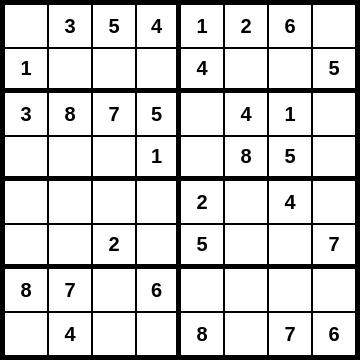
\includegraphics[width=0.3\textwidth]{../img/8x8sudoku.jpg}
   \caption[Strukura projektu]{Classic 8x8}
   \label{fig:8x8Sudoku}
\end{figure}

V programu je mřížka reprezentovaná pomocí dvourozměrného pole celých čísel o velikosti NxN specifikované nahoře. Prázdná pole jsou reprezentována pomocí -1. Pro reprezentaci celé

\subsubsection{ClassicX}
Pravidla u tohoto typu jsou stejná jako u klasického sudoku, nicméně platí zde, že číslo se v hlavní a vedlejší diagonále mřížky musí vyskytovat právě jednou. Například takto vypadá diagonální sudoku pro stejnou velikost 8x8.

\begin{figure}[H]
   \centering
   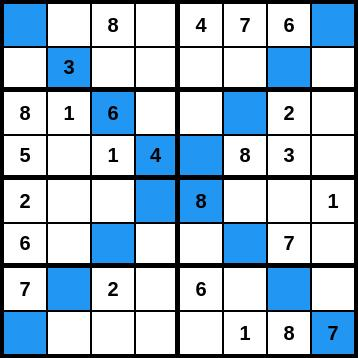
\includegraphics[width=0.3\textwidth]{../img/8x8DiagSudoku.jpg}
   \caption[ClassicX 8x8]{ClassicX 8x8}
   \label{fig:8x8DiagSudoku}
\end{figure}

\subsubsection{Jigsaw}
Tento typ se vyznačuje tím, že sekce zde nemají obdélníkový tvar. V každé sekci se však musí vyskytovat každé číslo právě jednou. Takto vypadá příklad pro jigsaw 9x9:

\begin{figure}[H]
   \centering
   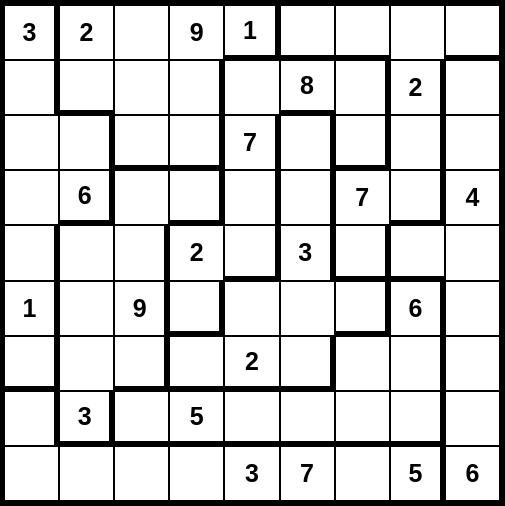
\includegraphics[width=0.3\textwidth]{../img/9x9jigsaw.jpg}
   \caption[Jigsaw 9x9]{Jigsaw 9x9}
   \label{fig:9x9jigsaw}
\end{figure}

V programové reprezentaci nám zde přibývají dvě proměnné:
\begin{itemize}
   \item \texttt{areaPointersGrid} -- dvojrozměrné pole o stejné velikosti jako mřížka obsahující prvky 1 - N. Tyto prvky označují číslo sekce, které daný index náleží
   \item \texttt{areasLists} -- každá sekce má v tomto listě 1 list obsahující objekty tvaru {row, col}. Dá se vytvořit z \texttt{areaPointersGrid} a slouží k rychlému zkontrolování, zda se v dané sekci nevyskytuje nějaké číslo dvakrát.
\end{itemize}

\subsubsection{Samurai}
Samurai sudoku je složeninou pěti samostatných mřížek, které jsou spojeny jednou sekcí. V této spojovací sekci musí čísla splňovat pravidla obou spojovaných mřížek. V ostatních případech splňuje pouze pravidlo jedné. Pro tento typ a samurai mixed je však zatím v aplikaci pouze minimální podpora.

\begin{figure}[H]
   \centering
   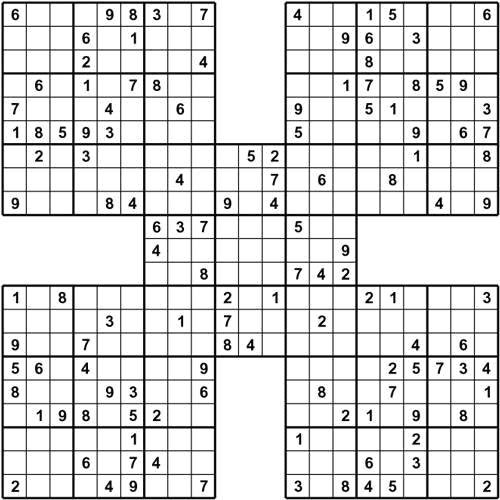
\includegraphics[width=0.5\textwidth]{../img/9x9samurai.png}
   \caption[Samurai 9x9]{Samurai 9x9}
   \label{fig:9x9samurai}
\end{figure}

\subsubsection{Samurai Mixed}
Tento typ je prakticky totožný s typem samurai, nicméně platí, že jednotlivé mřížky mohou být různými variantami. Jedna z variant např. tedy může být jigsaw, zatímco jiná ClassicX. Platí však, že pokud je jedna z variant Jigsaw, musí být spojovací sekce čtverec.

\section{Řešení}
Řešení sudoku je v kódu implementováno pomocí kódu v souboru \textit{solvers.js}. Jedná se o klasický backtrackingový algoritmus pracující na principu prohledávání do hloubky. Popis algoritmu:
potřebné proměnné:
\begin{itemize}
   \item N=velikost mřížky
   \item mr=mřížka -- dvourozměrné pole NxN
   \item
\end{itemize}
\begin{algEnumerate}
   \item začni na souřadnicích 0, 0,
   \item pokud sloupec > N, sloupec = 0, řádek++
   \item pokud řádek === N -- ulož řešení a ukonči rekurzi
   \item číslo -- pro všechna čísla od 1 do N:
   \begin{algEnumerate}
      \item zkontroluj, zda dané číslo může být položena na mr[řádek][sloupec]
      \item pokud ano, skoč na krok 2
   \end{algEnumerate}
   \item vlož -1 na mr[řádek][sloupec] (backtrack)
\end{algEnumerate}

Tímto způsobem dojde k nalezení všech řešení daného sudoku. Rekurze vždy skončí buď podmínkou v kroku č. 3, popř. doběhnutím metody až za krok 5. Složitost daného algoritmu je $O(M^{N})$, kde \textit{M} je počet možných dosazovaných čísel a \textit{N} počet políček, za které dosazujeme.

Tato složitost vůbec není dobrá a již pro sudoku 16x16 při určitém čísle \textit{N} již trvá řešení několik minut. Na tomto problému bych do maturitní práce rád zapracoval a vytvořil algoritmus, který řeší sudoku efektivně pokud možno až do velikosti 25x25.

Řešící metoda \textit{solveGeneral} v aplikaci přebírá jako parametr list callbacků, které spouští, aby zkontrolovala, zda může na dané políčko položit dané číslo. Jednotlivé sudoku čtvercového typu (mimo samurai) tedy této metodě předají příslušné callbacky a ona daný typ vyřešní. Není tedy třeba psát speciální solver pro každý typ, stačí pouze napsat vstupní metodu, která metodě \texttt{solveGeneral} předá příslušné callbacky (např. metoda \texttt{startSolvingClassic})

Všechna nalezená řešení jsou poté vložena do pole, které bylo metodě předáno jako argument.

\section{Generování}
Program dokáže kromě vyřešení sudoku také zadání vygenerovat. Za validní zadání považujme takovou mřížku, která má právě jedno řešení.

Algoritmus generování probíhá ve dvou oddělených fázích. V té první dojde k vytvoření validního řešení sudoku pro danou variantu. V té druhé z tohoto řešení odstraníme \textit{N} čísel, kde \textit{N} je určeno požadovanou složitostí a kontrolujeme, zda má tato mřížka právě jedno řešení.

\subsection{Tvorba validní mřížky}
Tvorba validní mřížky není až tak jednoduchý úkol, jak by se na první pohled mohlo zdát. Ve skutečnosti je svou složitostí na stejné, ne-li vyšší úrovni než řešení sudoku.

Na tvorbu je použit upravený algoritmus řešení:
\begin{algEnumerate}
   \item začni na nultém políčku
   \item pokud sloupec > N, sloupec = 0, řádek++
   \item pokud řádek === N -- ulož řešení a ukonči celý běh metody (zde stačí jen 1 řešení)
   \item pro všechna čísla, která se na políčku mohou nacházet v \textbf{náhodném pořadí}:
   \begin{algEnumerate}
      \item umísti dané políčko
      \item vyškrtni zapsané číslo z možností pro políčka v daném řádku, sloupci, boxu / diagonále, na kterých ještě není žádné číslo...
      \item jdi na krok 2 s dalším prvkem v pořadí (rekurze jako v předchozím případě)
      \item vlož zpět zapsané číslo z možností pro políčka v daném řádku, sloupci, boxu / diagonále... (rekurze skončila, dané číslo nemůžeme na daném čísle mít -- čištění)
   \end{algEnumerate}
\end{algEnumerate}

V programu je přidána proměnná \texttt{possibleNumbersGrid}, což je trojrozměrné pole o velikost NxNx(N+1). každý \texttt{possibleNumbersGrid}[řádek][sloupec] obsahuje list o N+1 prvcích. Tyto prvky reprezentují, kolikrát je dané číslo na dané pozici ohroženo. Např. pokud je \texttt{possibleNumbersGrid}[řádek][sloupec][2] = 3, poté to znamená, číslo 2 na pozici řádek, sloupec je invalidní ze 3 důvodů -- např. ve stejném řádku je 2, sloupci a boxu. Pokud je zde 0, poté sem číslo položit můžu, pokud něco jiného, tak nesmím.

Na první pohled by si člověk mohl říct, že by vlastně šlo pustit sudoku solver, který pouze vybírá náhodná čísla místo sekvenčního postupu 1 až N na prázdné mřížce, a že není třeba vytvářet nový kód. To by sice šlo, avšak toto řešení je více optimalizované, jelikož škrtání možných čísel na daném políčku se provádí pouze pro políčka, která ještě nejsou obsazena. Pro obsazená čísla by to totiž nemělo smysl, jelikož v backtrackingu jsou odebírány až po prvku, kvůli kterému se škrtá. Samotný způsob hledání je navíc už z principu více optimalizovaný, jelikož škrtání čísel znamená jeden průchod všemi sektory, kterými se má projít, zatímco solver tyto sektory musí projít pro každé číslo, které kontroluje.

\subsection{Tvorba zadání}
Algoritmus na tvorbu zadání je následující:
\begin{algEnumerate}
   \item vygeneruj validní mřížku pro daný typ sudoku
   \item zjisti počet čísel, které je potřeba z mřížky odstranit na základě obtížnosti
   \item odstraň N náhodných políček ze mřížky
   \item vyřeš pro tuto novou mřížku. Pokud má 1 řešení, vrať ho, pokud má více než 1, jdi na krok 3
\end{algEnumerate}

Ačkoliv se pro těžké sudoku krok 3 několikrát v průměru opakuje, pro 9x9 sudoku se jich stále vygeneruje několik za sekundu.

\subsection{Tvorba varianty zadání}
Vygenerovanou mřížku lze navíc jednoduchými operacemi s kvadratickou časovou složitostí (v závislosti na velikosti mřížky) upravit do podoby, kterou, nedáte-li ji uživateli okamžitě, nebude schopen odlišit od původní mřížky. Konkrétně, z jedné mřížky můžeme vytvořit 5 806 080 takovýchto variant.

Operace, které můžeme provést jsou:
\begin{itemize}
   \item permutace čísel -- celkem $9!$ možností
   \item rotace matice -- 4 možnosti
   \item transpozice matice -- dle hlavní diagonály, vedlejší diagonály, osy x, osy y -- 4 možnosti
\end{itemize}

Při kombinaci těchto možností vzniká pokaždé odlišné sudoku. Celkem tedy můžeme mít $9! * 4 * 4 = 5 806 080$ možných variant. O vytváření těchto variant se stará kód v souboru \texttt{variationCreator}

\chapter{Architektura}

\begin{figure}[H]
   \centering
   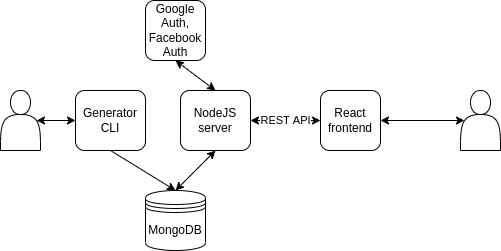
\includegraphics[width=0.8\textwidth]{../img/architecture.png}
   \caption[Architektura]{Architektura}
   \label{fig:architecture}
\end{figure}

K programu je možné přistoupit ze dvou bodů. Tím prvním je klasický uživatelský přístup z frontendu (viz kapitola 3). Přes REST API komunikuje s backendem (viz kapitola 4). Pomocí tohoto API jsou zpřístupněny funkce jako získání zadání her, autentifikace, změna uživatelských údajů či práce s obchodem.

Tím druhým bodem je CLI interface pro generování her, který slouží k vytvoření her požadovaných uživatelem a jejich uložení do databáze.

Kód pro frontend a backend je pro přehlednost rozdělen do dvou oddělených souborů -- client a backend s vlastním package.json souborem. V production módu je poté možnost nechat obě dvě být poskytovány jedním serverem.

\section{Autentifikace}

Tato kapitola pojednává o samotném principu autentifikace v aplikaci. Pro specifikaci autentifikačních API endpointů viz 

Autentifikace je proces zjištění totožnosti uživatele. Aplikace dovoluje uživatelům autentifikovat se třemi různými způsoby:
\begin{itemize}
   \item Local -- Přihlášení na stránce pomocí emailu a hesla (vnitřní systém stránky, je nutná předchozí registrace v aplikaci)
   \item Google Auth (OAuth 2)
   \item Facebook Auth (OAuth 2)
\end{itemize}
Pro implementaci tohoto procesu na backendu bylo využito knihovny passport.js, která celý proces usnadňuje. Základ kostry byl použit z našeho dřívějšího projektu AvAvA\footnote{\bibentry{AvAvA}}, nicméně prošel velkým refactoringem a předěláním do databáze MongoDB.

Pro každou ze tří strategií je nutné zapsat kód, který se zavolá hned po přihlášení, tedy uložení do databáze - passport.use(...) a předat passportu clientId a secretId daného provideru.

Dále je potřeba implementovat metody serializeUser a deserializeUser, které se budou volat po popořadě při zapisování ID do sessioncookie a při získávání uživatele z databáze za pomoci ID získané ze sessioncookie.

Pro zjištění, zda je uživatel přihlášen je možné na kterékoliv z request objektů získat property req.user, ve které bude uložen výsledek posledního volání metody deserializeUser. V případě, že žádný uživatel není přihlášen, jeho hodnota je null.

\subsection{Local}
Aby tuto strategii mohl uživatel použít, musí se nejprve zaregistrovat. Mezi požadované údaje patří první a druhé jméno, email a dostatečně silné heslo. To by mělo obsahovat alespoň 8 znaků, alespoň 1 velké písmeno, alespoň 1 číslici a alespoň 1 speciální znak. Toto je validováno jak na frontendu, tak i backendu. 

Tento typ autentifikace se plně odehrává v rámci aplikace a registrovaný uživatel je uložen do MongoDB databáze. Platí přitom, že není možné zaregistrovat uživatele, pokud se v databázi již uživatel s daným emailem nachází. 

\subsection{OAuth 2}

Díky OAuth 2 protokolu je možné se autentifikovat prostřednictvím poskytovatelů společností Google a Facebook. Pro zprovoznění Google Auth, resp. Facebook Auth je nejprve nutné si v Google Console, resp. Facebook Devtools vytvořit nový projekt. Odtud se zkopíruje clientId a clientSecret.

Není zde rozdíl mezi registrací a loginem. Jestliže se uživatel přihlašuje poprvé, bude uživatel v databázi vytvořen, jestliže je přihlašuje po několikáté, bude přihlášen. 

Jestliže se při prvním přihlášení již v databázi nachází uživatel s daným emailem, je jeho záznam updatován o data z provideru. Daný uživatel se bude moci přihlásit jak svým původním způsobem, tak i novým způsobem. Data jako obrázek či první a druhé jméno zůstanou zachována z minula, aby vše bylo konzistentní. Uživatel se tedy může dostat do situace, kdy se může přihlásit ke stejnému účtu jak přes google, tak přes facebook, tak i pomocí local strategy

\begin{figure}[H]
   \centering
   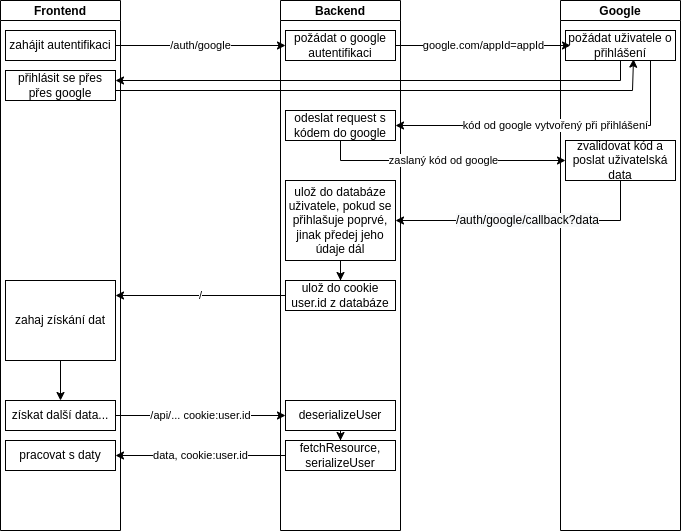
\includegraphics[height=9.5cm]{../img/googleAuth.png}
   \caption[Autentifikace přes Google Auth]{Autentifikace přes Google Auth}
   \label{fig:architecture}
\end{figure}

Na obrázku výše můžete vidět průběh autentifikačního procesu.
Nejprve uživatel musí autentifikaci zahájit, což udělá pokusem o získání nějakého chráněného obsahu.
Po odeslání žádosti z klienta na backend přesměruje uživatele na přihlašovací stránku Google.
V případě, že se student přihlásí poprvé, musí odsouhlasit, že povoluje programu využívat některé služby.
Při dalších návštěvách se už jen přihlásí.

Tím je proces autentifikace hotov a začíná proces autorizace programu u Googlu.
Aplikace tedy bude Google žádat, aby jí předal data o uživateli, která potřebuje.
To dělá v obdélníku “odelsat request s kódem do google”.
Pokud google vyhoví, zavolá callback, který mu byl nastaven při vytváření projektu v Google Console a odešle na něj chtěná data.

Následně je vytvořena session mezi frontendem a backendem. Každá zpráva odteď bude v hlavičce obsahovat cookie soubor s ID uživatele.

Po získání dat je uživatel přihlášen a může systém používat. Při odhlášení je session ukončena a už se dále user ID neposílá.

\subsection{Autorizace}

API endpointy je možné pomocí middleware requireAuth zajistit proti zavolání bez toho, aby byl uživatel přihlášen. Ostatní kontrolování, zda má uživatel na něco právo jsou subjektivní a jsou popsány u daného logického celku.

\chapter{Backend}

\begin{figure}[H]
   \dirtree{%
      .0 server.
      .1 src.
      .2 config.
      .2 database.
      .2 entities.
      .2 middleware.
      .2 routes.
      .2 service.
      .2 app.js.
      .2 generatorIndex.js.
      .2 index.js.
      .1 test.
   }
   \caption[Struktura souborů v src na backendu]{Struktura souborů na backendu}
   \label{fig:sqlClasses}
\end{figure}

Vstupním bodem aplikace je soubor \texttt{index.js} pro skript \texttt{npm start}. Na základě dat ze složky \texttt{config}, kde se nacházejí \texttt{env} a \texttt{.env.test} soubory s globálními proměnnými inicializuje server ze složky \texttt{app.js} a databázi ze složky database. Ve složce \texttt{routes} a \texttt{middleware} je vše, co zodpovídá za REST API v entities jsou poté základní objekty ukládající data, která jsou všude na serveru potřeba a ve složce \texttt{service} je poté samotná business logika aplikace. Soubor \texttt{generatorIndex.js} je poté vstupním bodem při generaci sudoku příkazem \texttt{npm run generate}. Kód \texttt{test} sousedící s src poté slouží k testování logiky z src. 

\section{Návrh}
Kód na backendu byl napsán tak za využití některých prvků z čisté architektury od Boba Martina \footnote{viz. \bibentry{CleanArchitecture}}. Kód dělím do několika vrstev od nejvyšší po nejnižší:
\begin{enumerate}
   \item vnější rozhraní (MongoDB interface, REST API, generator CLI)
   \item logické komponenty -- solvers, variationCreator, generators
   \item entity -- objekty reprezentující základní data naší aplikace (user, games). Jejich specifikace nemá smysl uvádět, jsou v kódu dobře popsané.
\end{enumerate}

Klíčové je pro ni využití návrhového vzoru \textbf{dependency injection (IOC)}. Tento způsob psaní je typický tím, že kód z nižší vrstvy nesmí být silně závislý na kódu z té vyšší. Silnou závislostí mám na mysli závislost vytvořenou importováním. Může na ni být závislý pouze slabě, tj. danou funkcionalitu předá vyšší vrstva té nižší při vytvoření jako parametr. Výhody tohoto přístupu:

\begin{itemize}
   \item Odolnost vůči změnám. Nižší vrstva není na ničem přímo závislá a tak při změnách v knihovnách či vyšších vrstvách a v případě správného použití adaptérů netknutá.
   \item Možnost vytvoření velmi spolehlivého jádra aplikace, které má výborné testové pokrytí. Díky tomu v této části prakticky nemohou vznikat chyby.
   \item Možnost jednoduše měnit závislosti. Např. v případě testování můžeme jednoduše předat našemu REST API serveru pomocí dependency injection testovou databázi. 
\end{itemize}

Entity a některé další části kódu -- např. databáze jsou vytvářené pomocí \textbf{tovární metody} -- např. makeUser({}). Ta vrátí objekt uživatele, k jehož vlastnostem je možné přistupovat pouze pomocí getterů, setterů a několika dalších metod. Zároveň provede kompletní validaci, aby se zabránilo, že objekt bude v invalidním stavu. 

Tím, že se s objektem pracuje pomocí metod je však zkomplikovaná práce při posílání dat na klienta přes REST API a posílání dat do databáze. To je však správně, v každém z těchto případů jsou potřeba pouze některé z vlastností, kterých může entita nabývat. Určitě bychom např. nechtěli na klienta posílat hash hesla z databáze. Je tedy před posláním potřeba entitu převést na objekt, který je pro danou situaci potřeba převést tento objekt na klasický javascript objekt bez funkcí. Na to použijeme návrhový vzor \textbf{adaptér}. Adaptéry pro API jsou přímo v entitách, zatímco adaptéry pro databáze jsou v databázových souborech.

Aby tomuto bylo předány potřebné závislostí, jsou tovární metody entit obaleny další tovární metodou buildMakeUser. Té jsou předány potřebné závislosti a její návratovou hodnotou je callback nane tovární metodu vyrábějící dané entity.

Tyto buildMake metody jsou volány z příslušného \texttt{index.js} souboru, který se nachází v dané složce. Takovýto index.js soubor se vyskytuje v každé složce, která odpovídá za nějakou oddělenou činnost a slouží k sjednocení přístupu k daným funkcím.  

\section{Databáze}

\begin{figure}[H]
   \dirtree{%
      .1 database.
      .2 models.
      .3 Games.
      .3 index.
      .3 User.
      .2 games.
      .2 index.js.
      .2 sessions.js.
      .2 users.js.
   }
   \caption[Soubory týkající se databáze]{Soubory týkající se databáze}
   \label{fig:sqlClasses}
\end{figure}

Jako databáze byla vybrána MongoDB, jelikož umožňuje pohodlnou reprezentaci polí a v programu se ani v dlouhodobém horizontu nevyskytuje mnoho použití relací. 

Ve složce models je specifikována struktura modelů pro vytvoření MongoDB kolekcí. V každém z těchto souborů se kromě modelu vyskytuje také metoda vytvářející daný databázový objekt z předané entity. Jedná se o návrhový vzor \textbf{adaptér}, jelikož databázové logice jsou předávány entity, nikoliv databázové objekty.

Mimo složku models jsou poté soubory obsahující různé metody, které nad těmito modely operují. Jedná se o metody jako \texttt{findRandomClassicGame} či \texttt{findUserByEmail}. Všechny tyto metody jsou poté exportovány ze soubory index.js, ve kterém se zároveň nastavuje celá mongo databáze. Jedná se o návrhový vzor \textbf{fasáda}, jelikož vytváříme zjednodušující vrstvu pro práci s databází.

Díky této zjednodušující můžeme kdykoliv databázi vyměnit a zbytek programu nebude nijak ochromen. Stačí nám poté pouze změnit implementaci těchto zmíněných fasádních metod.

\subsection{Modely}

\subsubsection{User}
Ve schématu se nachází: \texttt{first\_name}, \texttt{last\_name}, \texttt{email}, \texttt{coins\_count} (peníze uživatele), \texttt{profile\_picture\_link} (odkaz na obrázek profilovky), \texttt{auth} -- autentifikační data (\texttt{hash} hesla pro local, \texttt{id} + \texttt{accessToken} pro facebook a google)

\subsubsection{ClassicGame}
Ve schématu se nachází: \texttt{seed} -- mřížka se zadáním (dvojrozměrné pole NxN s -1 jako prázdnými místy), \texttt{solution} -- mřížka s řešením, \texttt{difficulty} -- obtížnost

Tato reprezentace je výhodná v tom, že sudoku, které pochází z databáze není nutné již řešit, jelikož řešení je zde již uloženo. Když si tedy na frontendu někdo vyžádá vyřešení dané úlohy, jednoduše se jen zobrazí \texttt{solution}. 

Tento model slouží jako základ pro většinu dalších modelů, protože většinou potřebují podobné typy na uložení.

Každý typ má vlastní tabulku hlavně z důvodů výkonnosti, aby při hledání daného typu hry nebylo nutné procházet i typy, které s ním vůbec nesouvisí, ale také z důvodu, že hry nemusí mít stejné schéma -- viz samurai a jigsaw.

\subsubsection{ClassicXGame}
Stejné schéma jako ClassicGame

\subsubsection{JigsawGame}
Schéma z classicGame, ale navíc \texttt{areaPointersGrid} (již vysvětleno dříve)

\subsubsection{SamuraiGame, SamuraiMixedGame}
solution a seed zde nejsou dvojrozměrné pole, ale objekty s vlastnostmi: \texttt{tl} (top left), \texttt{tr}, \texttt{m}, \texttt{bl}, \texttt{br} obsahující dvojrozměrná pole dané části.

\section{Specifikace REST API}
Tato kapitola se věnuje popisu REST API určené pro komunikaci mezi klientem a serverem.

\subsubsection{\color{apiblue}{POST -- /api/auth/register}}
\texttt{body: email, firstName, lastName, password} 

V případě, že uživatel předal všechny potřebné parametry, heslo je dost silné a v databázi se daný uživatel ještě nevyskytuje, je uživatel zaregistrován.

\subsubsection{\color{apiblue}{POST -- /api/auth/login}}
\texttt{body: email, password} 

V případě, že uživatel předal všechny potřebné parametry, uživatel se v databázi vyskytuje a heslo je správné, je uživatel přihlášen pomocí PassportJS.

\subsubsection{\color{apigreen}{GET -- /api/auth/google}}
Vstupní bod pro počátek google autentifikace -- dále mimo kontrolu aplikace až do vrácení dat od googlu. Ta jsou poté předána do PassportJS middleware

\subsubsection{\color{apigreen}{GET -- /api/auth/facebook}}
Vstupní bod pro počátek google autentifikace -- dále mimo kontrolu aplikace až do vrácení dat od facebooku. Ta jsou poté předána do PassportJS middleware

\subsubsection{\color{apiblue}{POST -- /api/auth/logout}}
Ukončí aktuální session

\subsubsection{\color{apigreen}{GET -- /api/user}}
Vrátí objekt aktuálního uživatele, pokud je přihlášen. Jestliže není, vrátí 401

\subsubsection{\color{apiblue}{POST -- /api/user/password}}
\texttt{body: oldPassword, newPassword} 
API endpoint pro změnu hesla uživatele. Pokud je oldPassword stejné jako staré heslo a newPassword je dostatečně silné, dojde ke změně hesla v databázi. Po získání zadání z databáze vytvoří variantu hry a tu poté odešle na klienta.

\subsubsection{\color{apigreen}{GET -- /api/games/classic}}
\texttt{body: size, difficulty} 
API endpoint pro vracení zadání typu classic o dané velikosti a složitosti. V případě, že pro dané zadání není v databázi žádný záznam, vrací 500. Po získání zadání z databáze vytvoří variantu hry a tu poté odešle na klienta.

\subsubsection{\color{apigreen}{GET -- /api/games/classicX}}
\subsubsection{\color{apigreen}{GET -- /api/games/jigsaw}}
\subsubsection{\color{apigreen}{GET -- /api/games/samurai}}
\subsubsection{\color{apigreen}{GET -- /api/games/samuraiMixed}}
to samé jako /api/games/classic, akorát pro jiné typy

\subsection{CLI pro generátor}
Tato aplikace podporuje i generování her, které trvá vygenerovat i delší dobu než je několik minut. Je proto dobrý nápad nenechat aplikaci generovat hru samotnou, ale nechat administrátora, aby sudoku nechal na požadavek manuálně vygenerovat. 

Generátor se zapíná na backendu příkazem \texttt{npm run generate}. 

Na začátku se uživatele zeptá na otázku: 
\begin{lstlisting}[breaklines, basicstyle=\tiny]
Which of these game types would you like to generate? Type only the number preceding name. Type only one!
1) Classic
2) ClassicX
3) Jigsaw
4) Samurai
5) Samurai mixed
\end{lstlisting}

Odpovědí by mělo být číslo daného typu. Pokud tomu tak není, zeptá se znovu. 

Následně se dle předaného typu zeptá na velikost. 
\begin{lstlisting}[breaklines, basicstyle=\tiny]
Select size of Classic
1) 4x4
2) 6x6
3) 8x8
4) 9x9
5) 10x10
6) 12x12
7) 14x14
8) 16x16
\end{lstlisting}
Opět se očekává číslo před pravou kulatou závorkou. Cokoliv jiného vyústí v zopakování otázky.

Následně je vyžádána obtížnost úlohy:
\begin{lstlisting}[breaklines, basicstyle=\tiny]
Select difficulty of Classic
1) easy
2) normal
3) hard
\end{lstlisting}

Úplně nakonec si CLI vyžádá počet sudoku na vygenerování (limitováno od 1 do 200 -- čísla vybrána arbitrárně na základě zkušenosti): 
\begin{lstlisting}[breaklines, basicstyle=\tiny]
How many games of type Classic with size 9x9 and difficulty hard (1-200)
\end{lstlisting}

Jakmile je vše vybráno, začne se daný počet generovat. Jakmile bude vždy 1 sudoku vygenerováno a uloženo, vypíše se uživateli zpráva:
\begin{lstlisting}[breaklines, basicstyle=\tiny]
49. sudoku generated and stored
50. sudoku generated and stored
\end{lstlisting}

Během tohoto generování může uživatel psát znova, jelikož se generátor vrací v nekonečné while smyčce na první dotaz. Není tedy třeba znovu skript spouštět. Jelikož se ukládání provádí asynchronně, není třeba na čekat, než se vše dogeneruje.

\subsection{Testy}
Na backendu bylo možné postupovat stylem test-driven development. Jádro tohoto postupu spočívá v tom, že se nejdříve napíše test a jeho výsledek a až následně se píše samotný kód. Ačkoliv jsem ke konci, hlavně u generátorů, byl nucen od tohoto testu upustit, mohu s jistotou tvrdit, že přes 85 procent backendu pokryto automatizovanými unit a integračními testy. 

Na testování byl použit framework Jest. Pro testování API knihovna supertest-session, což je wrapper pro supertest podporující session. Testy využívají testovací databázi, která má stejnou strukturu jako ta produkční, akorát je k jejímu jménu přidán postfix test. 

\begin{figure}[H]
   \dirtree{%
      .1 server.
      .2 jest.config.js.
      .2 test.
      .3 integration.
      .4 auth-profile-routes.test.js.
      .4 game-routes.test.js.
      .3 setup.
      .4 apiClient.js.
      .4 data.js.
      .4 helpers.js.
      .4 index.js.
      .4 testDBClient.js.
      .3 unit.
      .4 entities.
      .5 user.test.js.
      .4 solvers.test.js.
      .4 validations.test.js.
      .4 variations.test.js.
      .3 setup-tests.js.
   }
   \caption[Souborová struktura testů]{Souborová struktura testů}
   \label{fig:sqlClasses}
\end{figure}

Soubor \texttt{jest.config.js} zajišťuje správnou interpretaci absolutních cest na backendu, kterého je docíleno pomocí závislosti na knihovně sexy-require. Zároveň specifikuje setup file -- \texttt{setup-tests.js}, jehož role je připravit proměnné prostředí (\texttt{.env.test})

Ve složce setup se nacházejí soubory s často používaným kódem -- např. vkládání testovacích prvků do databáze (\texttt{testDBClient.js}), časté API requesty (\texttt{apiClient.js}), opakující se testovací data (\texttt{data.js}) či různé pomocné metody jako kontrola rovnosti mřížek sudoku (\texttt{helpers.js}). To vše je exportováno z index.js, kde se vše kombinuje a vytváří se zde instance testovacího serveru.

\subsection{Unit testy}
Unit testy slouží k testování jedné, často velmi malé funkcionality. Testují se zde správná funkčnost řešení sudoku (\texttt{solvers.test.js}), správná funkčnost variačních technik jako transpozice apod. \texttt{variations.test.js} či správná funkčnost validací -- silné heslo či nikoliv (\texttt{validators.test.js}). 

Zároveň se zde také testuje, zda správně funguje vytváření entit a zda je nelze dostat do nekonzistentního stavu. Zatímco u uživatele na toto je speciální soubor (\texttt{user.test.js}), u her je toto prováděno implicitně, jelikož metody na vytváření entit jsou použity v souboru \texttt{data.js} kdyby tedy bylo něco v nepořádky, testy by selhaly zde.

\subsection{Integrační testy}
Integrační testy testují několik komponent dohromady. V případech této aplikace se jedná o testování API, v jehož rámci zároveň dochází i k testování databáze.

Pro testování API pro autentifikaci a uživatelské akce je použit soubor (\texttt{auth-profile-routes.test.js}), zatímco pro herní API je použit \texttt{game-routes.test.js}




\chapter{Frontend}

Frontend byl napsán v Javascriptu za pomoci knihovny ReactJS. Vzhled byl zajištěn pomocí preprocessoru SASS. Zároveň bylo masivně využito knihovny Material-UI, která zajišťuje příjemný jednoduchý vzhled.

\section{Struktura souborů}

Následující sekce popisuje strukturu souborů clienta.

\begin{figure}[H]
   \dirtree{%
      .1 client.
      .2 package.json.
      .2 jsconfig.json.
      .2 public.
      .2 src.
   }
   \caption[Struktura souborů frontendu]{Struktura souborů frontend}
   \label{fig:frontendStructure}
\end{figure}

SSoubor \texttt{package.json} obsahuje informace o použitých knihovnách. Soubor \texttt{jsonconfig.json} je soubor struktury konfiguračního projektu pro typescript, který ovšem používáme i bez typescriptu, jelikož nám umožňuje používat absolutní adresování v projektu. Složka \texttt{public} je vygenerovaná od utility create-react-app a slouží pro vygenerování React stromu do HTML souboru. Složka \texttt{src} poté obsahuje veškerý náš kód.

\subsubsection{Src}
\begin{figure}[H]
   \dirtree{%
      .1 client.
      .2 src.
      .3 api.
      .3 assets.
      .3 components.
      .3 config.
      .3 redux.
      .3 games.js.
      .3 history.js.
      .3 index.svg.
      .3 routes.js.
      .3 setupProxy.js.
   }
   \caption[Struktura souborů frontendu -- src]{Struktura souborů frontend -- src}
   \label{fig:frontendStructureSrc}
\end{figure}
Zdaleka nejdůležitější je ovšem src složka, která obsahuje samotný kód.
Vstupním bodem je zde \texttt{index.js}, který renderuje aplikaci pomocí ReactDOM. Soubor \texttt{routes.js} obsahuje text jednotlivých cest na frontendu, aby byly centrallizované na jednom místě. Soubor \texttt{history.js} obsahuje objekt history pro connected-react-router. 

Soubor \texttt{games.js} poté obsahuje veškeré informace pro centralizaci informací o různých herních typech. Na frontendu totiž není možná stejná práce s entitami jako na backendu (hlavně kvůli Reduxu), popř. je to silně nevýhodné. K datům je zde lepší přistupovat nikoliv pomocí getterů a setterů, ale přímo (viz Redux). Informace je tedy nutné centralizovat jinde než entitách.

\subsubsection{Api}
Ve složce api se nachází veškerý kód potřebný ke komunikaci s REST API pomocí klentu axios.

Jelikož při developmentu nejsou backend a frontend na jednom portu, dochází ke CORS erroru. Na jeho vyřešení byla implementována http proxy (soubor \texttt{setupProxy.js}), která veškeré specifikované requesty přesouvá na port 5000 se stejnou adresou. Jedná se o návrhový vzor \textbf{proxy}

\subsubsection{Components}

\begin{figure}[H]
   \dirtree{%
      .1 client.
      .2 src.
      .3 components.
      .4 atoms.
      .4 molecules.
      .4 organisms.
      .4 pages.
      .4 templates.
      .4 environment.
   }
   \caption[Struktura souborů -- components]{Struktura souborů -- components}
   \label{fig:frontendStructureComponentes}
\end{figure}
Složka components obsahuje veškeré komponenty, ze kterých je apliakce složena. Je zde ctěna architektura \textbf{atomic design}. Ten říká, že komponenty je možné rozdělit do 5 skupin:
\begin{itemize}
   \item \texttt{atoms} -- prvky, které používá více různých komponentů jiné funkce a nelze je dále dělit -- tlačítka, ikonky (zde se kvůli silnému využití material ui téměř nevyskytují)
   \item \texttt{molecules} -- skupiny atomů, které používá více komponentů jiné funkce (zde se kvůli silnému využití material ui téměř nevyskytují)
   \item \texttt{organisms} -- skupiny molekul a atomů, které používá alespoň 1 stránka -- většina komponent aplikace
   \item \texttt{templates} -- šablona pro stránku (např. NormalPage pro stránky se Sidebarem a Navbarem)
   \item \texttt{pages} -- stránky dostupné na jednotlivých routách
\end{itemize}
Složka \texttt{environment} poté obsahuje pouze \texttt{App.js} komponentu, která dává vše dohromady a utilizuje connected-react-router

\subsubsection{Assets}

\begin{figure}[H]
   \dirtree{%
      .1 client.
      .2 src.
      .3 assets.
      .4 img.
      .4 styles.
      .5 atoms.
      .5 environment.
      .5 helpers.
      .5 organisms.
      .5 templates.
      .5 index.scss.
   }
   \caption[Struktura souborů frontendu -- assets]{Struktura souborů frontend -- assets}
   \label{fig:frontendStructureAssets}
\end{figure}
Ve složce assets se nachází vše, co se týká stylů, obrázků a fontů potřebných pro projekt.
Kód napsaný v assets/scss se díky preprocessoru zkompiluje do css souborů do složky assets/css, které se poté odesílají spolu s HTML souborem.

Styly kopírují strukturu atomic designu, přičemž navíc je zde složka helpers, ve které jsou souboru pro pomocné SASS funkce, proměnné a mixiny.

\subsubsection{Utils}
Ve složce service se nacházejí služby, které mohou využívat jakékoliv komponenty.
Jedná se o různé druhy validací, notifikace apod.

Ve složce views sídlí jednotlivé stránky.
Ty jsou v ní dále rozděleny podle toho, do jaké kategorie spadají.
Zde jsou vidět všechny tři kategorie.
Ve složce Other se poté nacházejí stránky z templatu pro případ, kdy by bylo možné někdy použít některé z template komponentů.

\section{Redux}

Redux je framework, který dovoluje různým React komponentům sdílet stav pomocí tzv. Redux store. Obdoba návrhového vzoru \textbf{kontext} ze Spring frameworku.
V případě, že nějaký komponent potřebuje přistoupit k nějaké části storu, tak se napíše metoda mapStateToProps a jednotlivé proměnné jsou poté předány jako properties jednotlivým komponentám.
V případě, že dojde ke změně redux storu, dojde k překreslení daného komponentu.

Se storem je možné manipulovat pouze pomocí tzv. akcí.
Jedná se o objekty, které obsahují jméno a payload.
Tyto akce se nacházejí ve složce actions v odlišných souborech pro uživatelské akce, akce s projekty, akce s uživateli a frontendové akce.
Tyto akce mohou být tzv. dispatchnuty, čímž se dostanou k reducerům.

\begin{figure}[H]
   \dirtree{%
      .1 client.
      .2 src.
      .3 redux.
      .4 actions.
      .4 reducers.
      .4 store.js.
   }
   \caption[Struktura souborů frontendu -- redux]{Struktura souborů frontend -- actions}
   \label{fig:frontendStructureSrc}
\end{figure}

Reducer je metoda, která na základě jména a payloadu předané akce určí, co se má stát s Redux storem.
Tento způsob změny stavu se může zdát zvláštní, každopádně zajišťuje vynikající škálovatelnost systému.
Aktuálně se zde nacházejí dva reducery -- \texttt{user} pro zajištění dat o uživateli a \texttt{games} pro zajištění dat o hrách. 

Na games reduceru se nachází několik důležitých proměnných. První z nich je currentlyPlayed. Ta obsahuje řetězec označující typ aktuálně hrané hry.

Poté se zde nachází pro každý typ hry objekt, do něhož se ukládají data pro aktuálně hranou hru. Je tedy možné mít více rozehraných typů her najednou a volně mezi nimi přeskakovat. 

Akce mohou být i asynchronní, což se např. hodí pro případ, kdy chceme poslat request na API a jakmile získáme výsledek, tak udělat se získanými daty nějakou akci. Na toto používáme redux-thunk.

Jednotlivé komponenty poté přistupují k datům pomocí \texttt{useSelector} hooku.

Hlavní účel využití Reduxu v projektu je tedy zpracování dat, které se získají z API do podoby, se kterou mohou komponenty pracovat a poskytnutí možnosti tato data měnit s okamžitými účinky na frontendu.

\section{Přehled funkcí}
Tato kapitola ukazuje základní přehled o funkcích frontendu

\subsection{Registrace}
Registrační stránka obsahuje možnost registrovat se pomocí Googlu a Facebooku pomocí dvou kulatých tlačítek, popř. pomocí formuláře. Je zde také odkaz na přihlašovací stránku vpravo dole.

Je zde použito validace, takže se nemůže stát, že by uživatel odeslal invalidní formulář. Toho je docíleno pomocí knihoven React Formik a Yup.
\begin{figure}[H]
   \centering
   \fbox{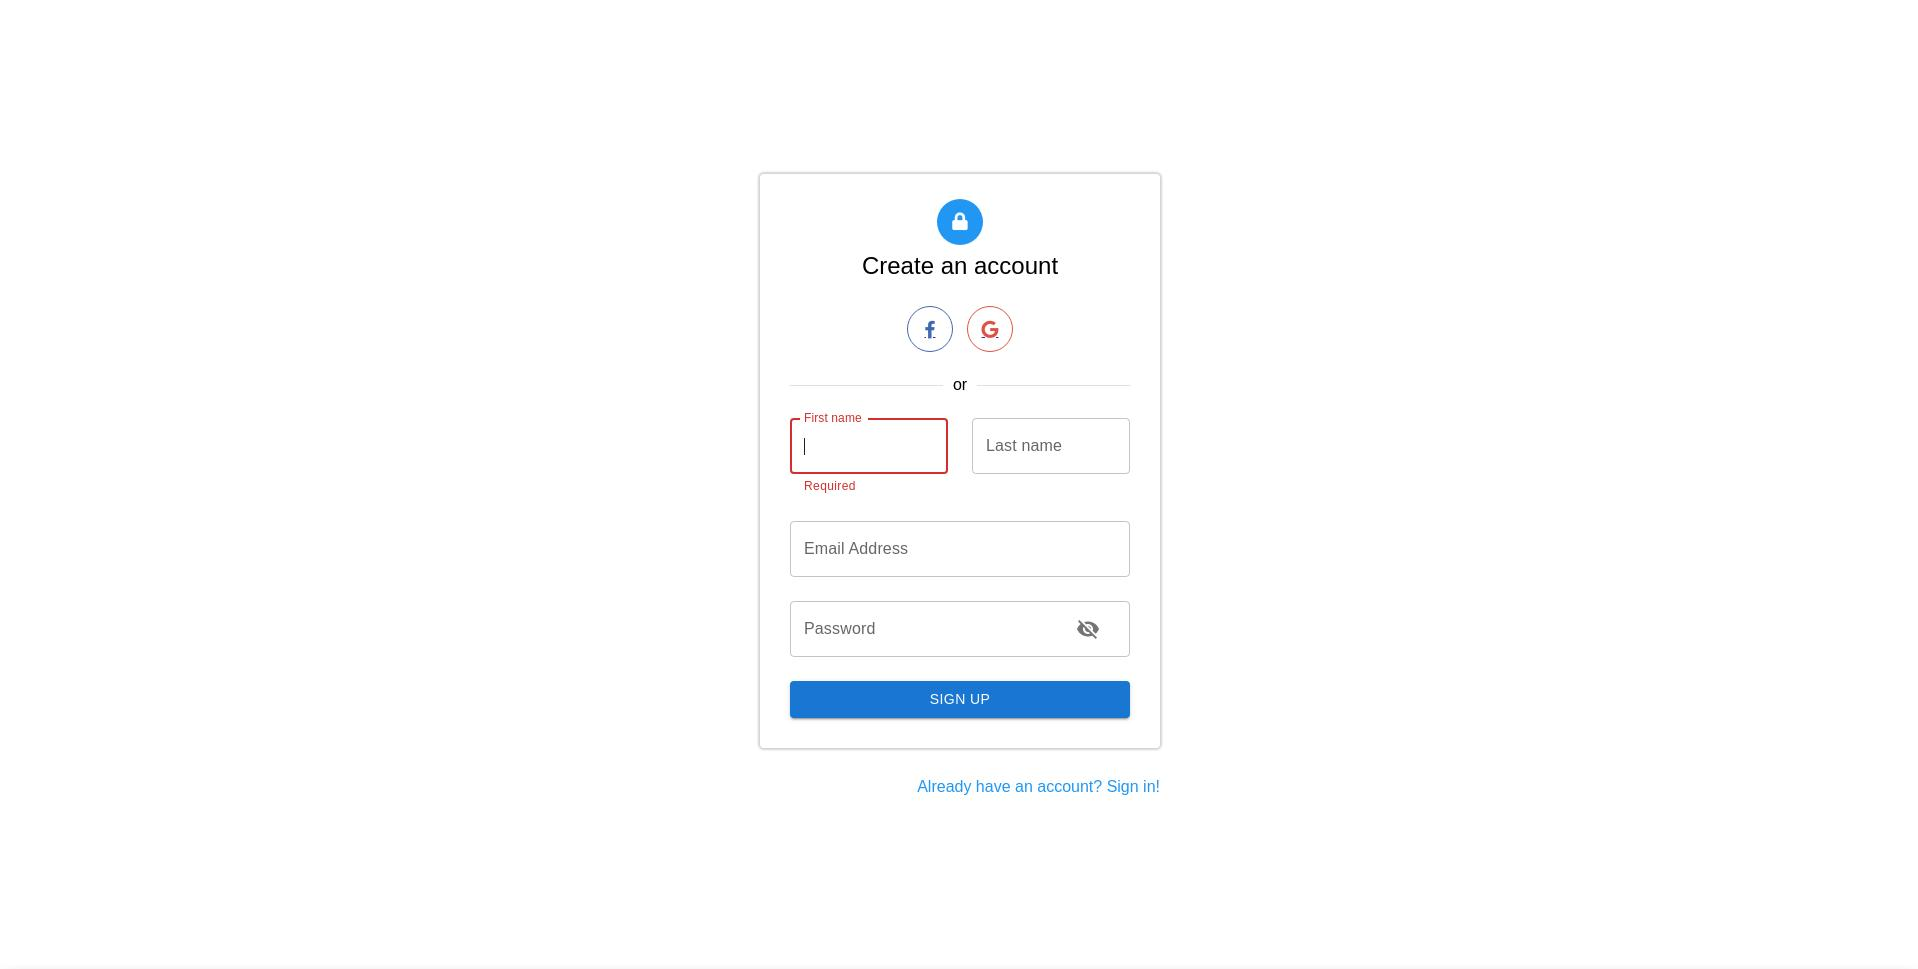
\includegraphics[width=0.8\textwidth]{../img/SignupPage.jpg}}
   \caption[Registrační stránka]{Registrační stránka}
   \label{fig:architecture}
\end{figure}

\subsection{Přihlášení}
Přihlašovací stránka obsahuje možnost přihlásit se pomocí Googlu a Facebooku pomocí dvou kulatých tlačítek, popř. pomocí formuláře. Je zde také odkaz na registrační stránku vpravo dole.

I zde je použito validace, takže se nemůže stát, že by uživatel odeslal invalidní formulář. Toho je docíleno pomocí knihoven React Formik a Yup. Remember-me a forgot password funktionality však zatím implementovány nejsou, takže jsou spíše na okrasu.
\begin{figure}[H]
   \centering
   \fbox{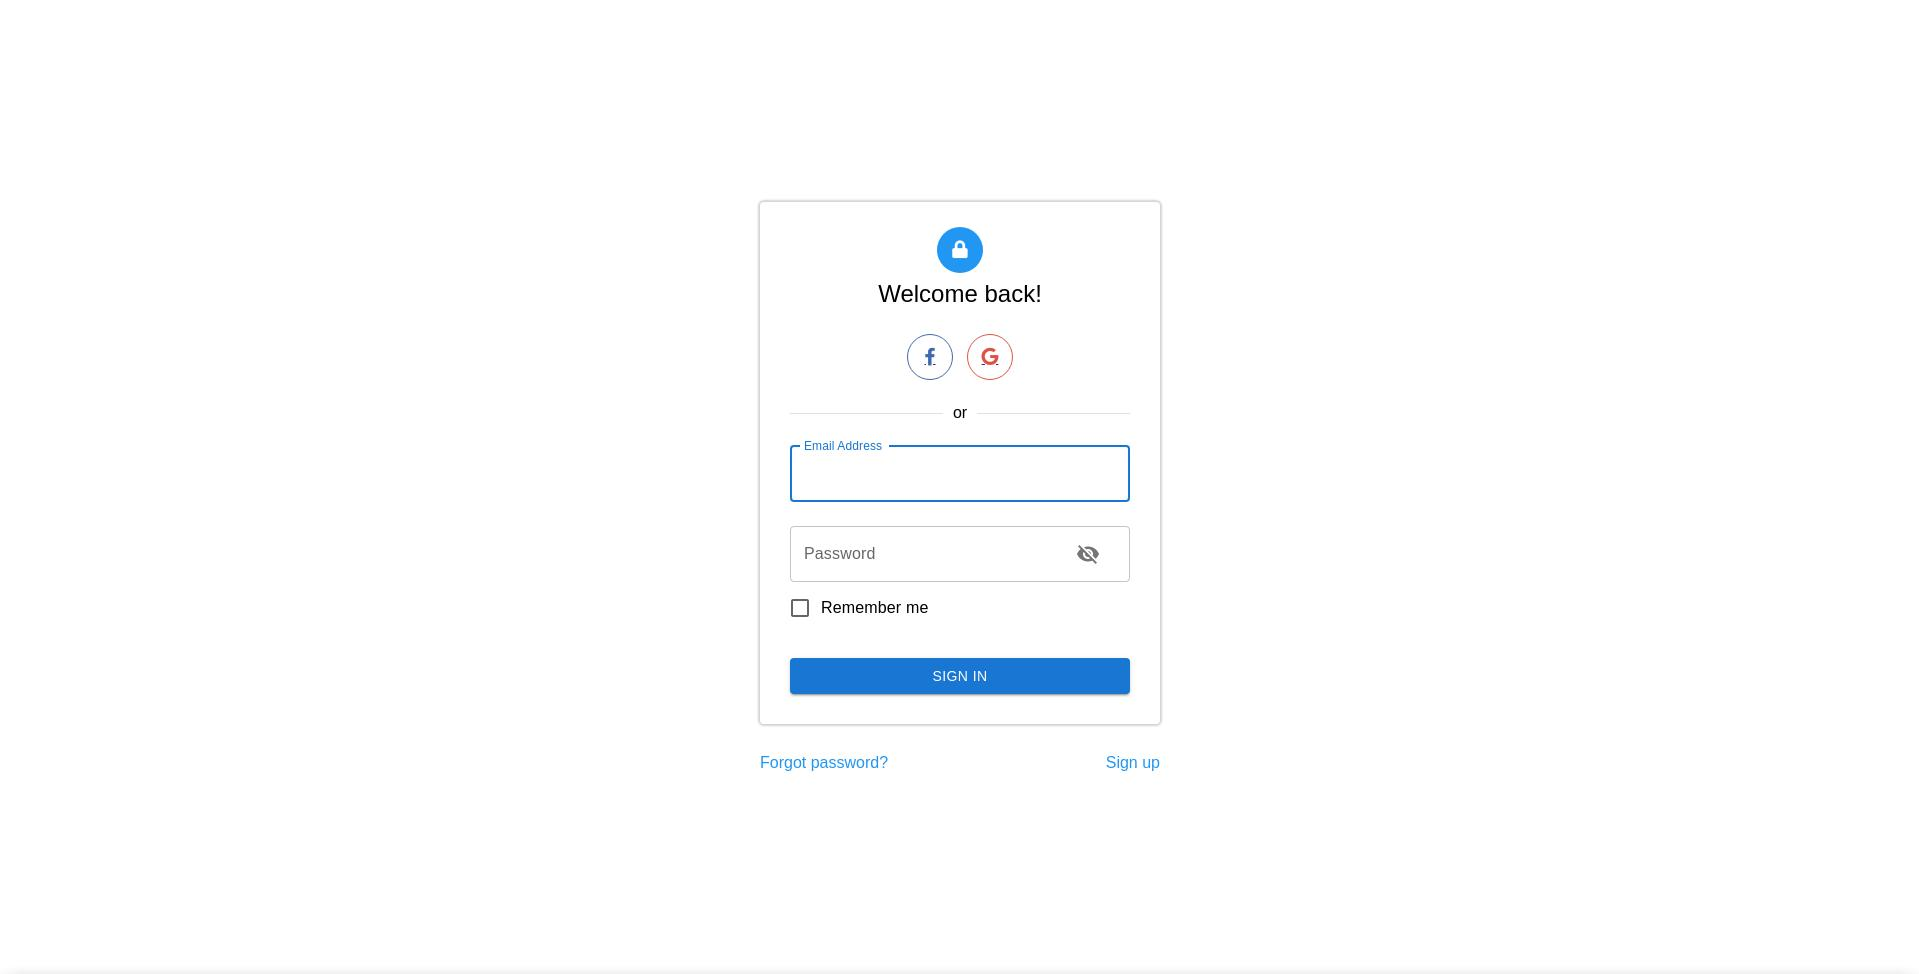
\includegraphics[width=0.8\textwidth]{../img/LoginPage.jpg}}
   \caption[Přihlašovací stránka]{Přihlašovací stránka}
   \label{fig:architecture}
\end{figure}

\subsection{Normální stránka}
\begin{figure}[H]
   \centering
   \fbox{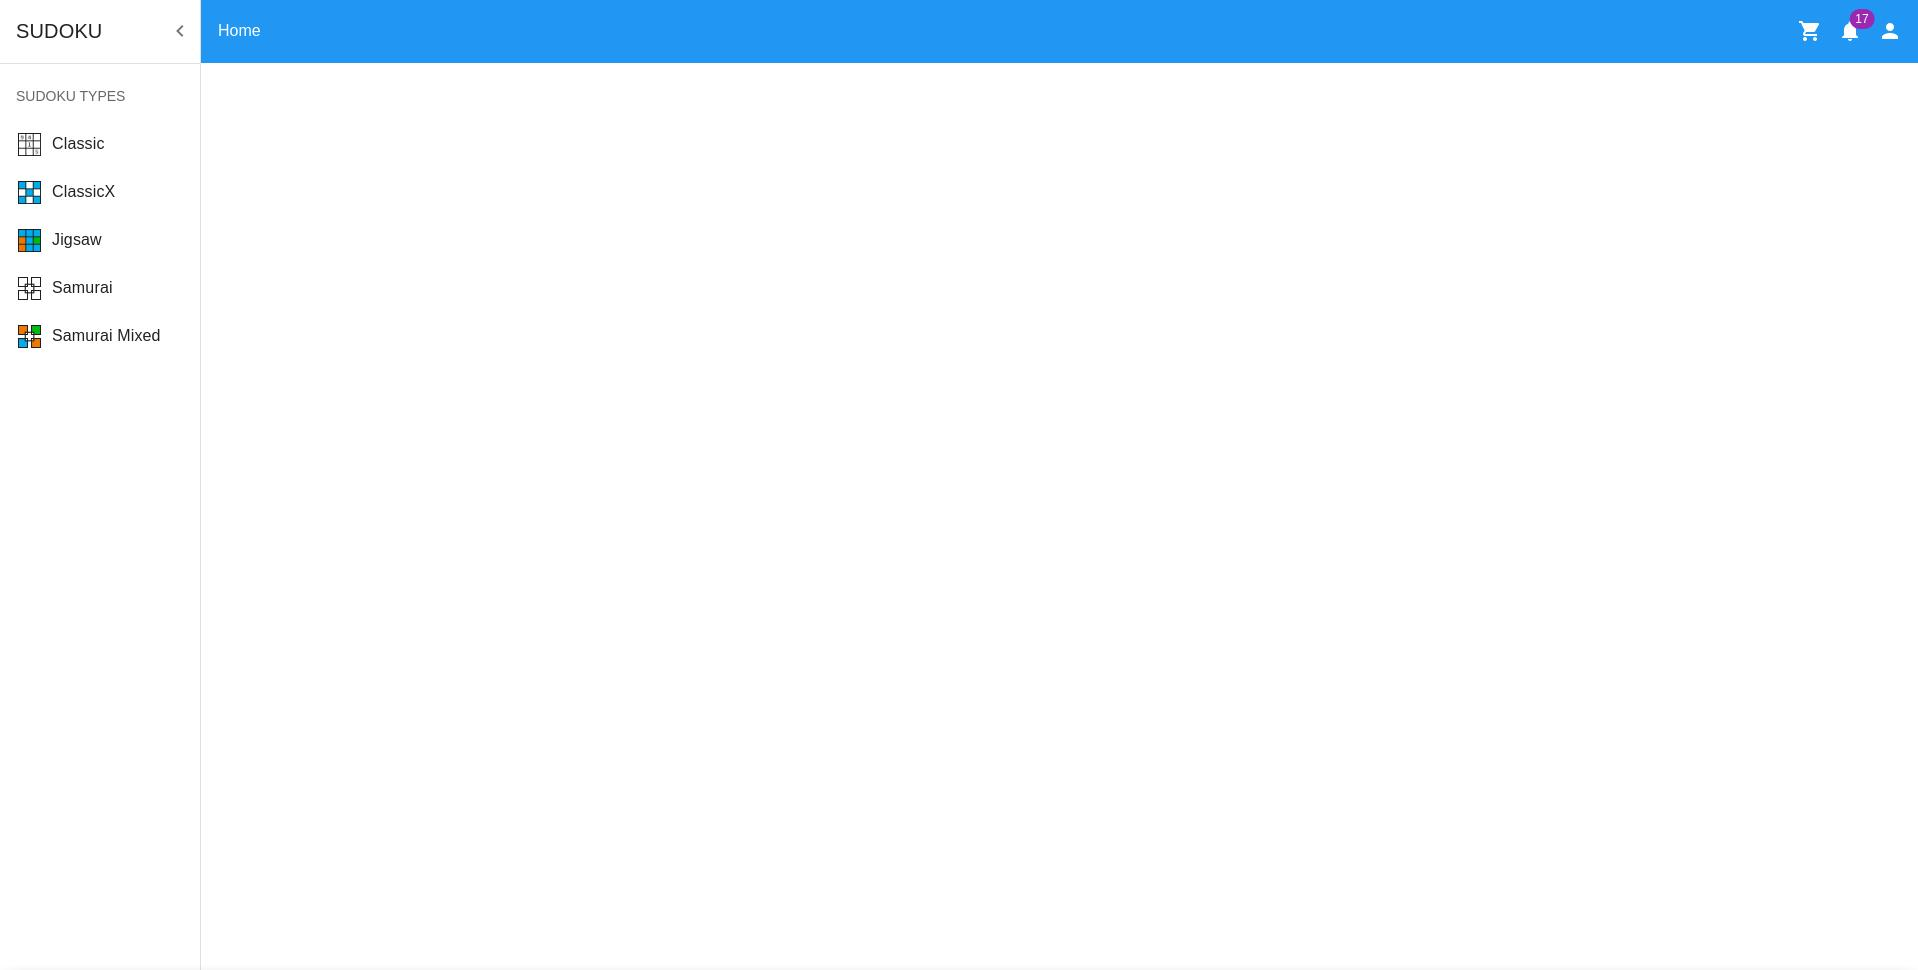
\includegraphics[width=0.8\textwidth]{../img/HomePage.jpg}}
   \caption[Přihlašovací stránka]{Přihlašovací stránka}
   \label{fig:architecture}
\end{figure}

Normální stránka obsahuje navbar obsahující informaci, jakou hru aktuálně uživatel hraje (pokud žádnou nehraje, nezobrazí nic). a také uživatelské informace. Jestliže uživatel není přihlášený, zobrazí se ikona anonymního uživatele, jelikože se načítá, zobrazí se spinner a jestliže je přihlášený, zobrazí se něco takového: 

\begin{figure}[H]
   \centering
   
\includegraphics[width=0.3\textwidth]{../img/vladimirIcon.jpg}
   \caption[Přihlášený uživatel]{Přihlášený uživatel}
   \label{fig:architecture}
\end{figure}

Stránka obsahuje také zatahnutelný sidebar, pomocí kterého se vybírají hry. Při kliknutí na jednu z možností se zobrazí takovéto menu:

\begin{figure}[H]
   \centering
   \fbox{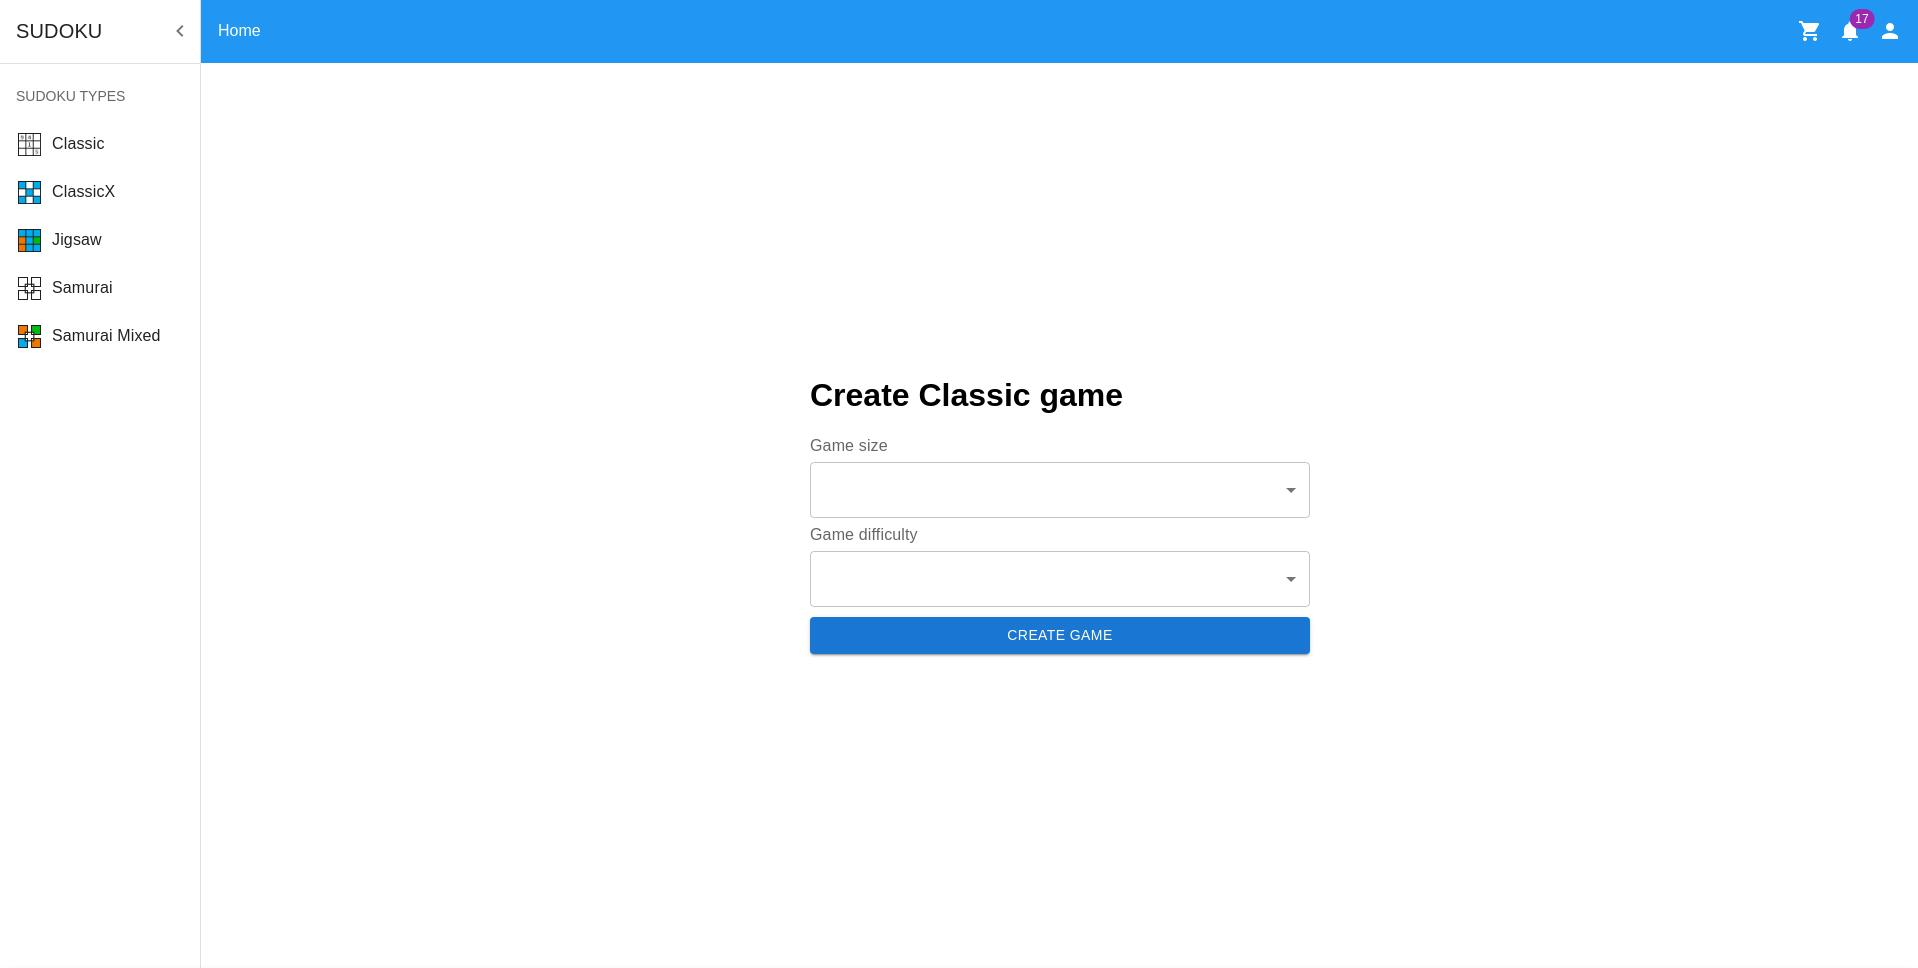
\includegraphics[width=0.8\textwidth]{../img/gameMenu.jpg}}
   \caption[Přihlašovací stránka]{Přihlašovací stránka}
   \label{fig:architecture}
\end{figure}

Pomocí select boxů se zde dají nastavit velikost hraného sudoku a obtížnost. Po nastavení a kliknutí na modré tlačítko se dispatchne akce, která se serveru zeptá na daný typ sudoku. Jestliže dostane odpověď s daty, vloží do Redux storu na dané místo data pro hru a je možné hrát. Jestliže dostane negativní odpověď, dispatchne se notifikace, že pro dané nastavení není na serveru žádné sudoku, popř. jinou chybu. Do doby, než přijde odpověď se zobrazuje spinner.

\subsection{Hraní různých typů her}

Aplikace dovoluje uživateli sudoku hrát a zároveň mu je schopna napovídat, zda porušuje pravidla sudoku. Takto např. vypadá, když je poruší: 

\begin{figure}[H]
   \centering
   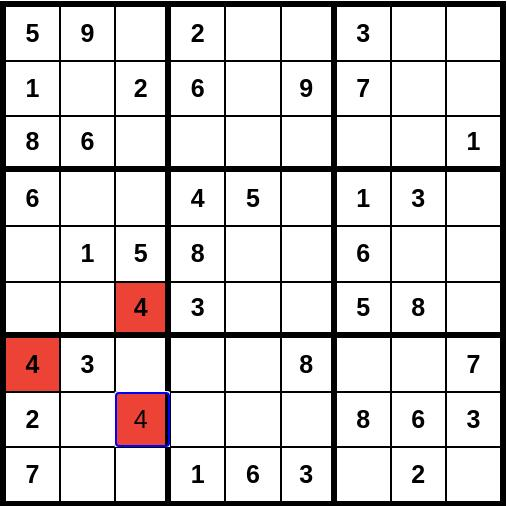
\includegraphics[width=0.3\textwidth]{../img/badSudoku.jpg}
   \caption[Porušení pravidel sudoku]{Porušení pravidel sudoku}
   \label{fig:architecture}
\end{figure}

Fokus mezi jednotlivými políčky je možné předávat pomocí šipek či myši. Čísla jsou vyplňována klávesnicí a prázdné políčko je vyplněno pomocí delete či backspace. Není možné přepsat předvyplněné políčko. 

Tohoto všeho se dosahuje pomocí dispatchování změny hracích dat do reduxu pokaždé, co se přidá nové číslo. Musí se tedy vyrenderovat celé sudoku znovu. To sice vypadá jako plýtvání výkonem, nicméně pro každý tah se musí celé sudoku zvalidovat a v případě nekonzistence se musí ukázat nepřesnosti. Tak jako tak se tedy musí celá mřížka přerenderovat. 

Zároveň je tento postup dobrý v tom, že je díky němu možné jednoduše přidat tlačítkový interface, kdy při kliknutí na tlačítko by se na fokusované políčko vložilo dané číslo.

\chapter*{}
\pagenumbering{roman}
\setcounter{page}{6}
\chapter*{Závěr}
\addcontentsline{toc}{chapter}{Závěr}
Z práce se povedlo splnit vše z povinné části a kromě toho byly přidány některé funkce, které jsem původně nezamýšlel, jako např. možnost pokračovat v uložené hře. Ačkoliv se jedná o projekt, který svým účelem nemá sám o sobě praktické použití, rozhodně mělo jeho vypracování smysl, jelikož mi poskytlo některé nové znalosti o testování, návrhových vzorech a dalších technologiích. Kromě toho jsem zde vytvořil znovu-použitelné komponenty, které je možné kdykoliv použít v programování jiných projektů (autentifikace, komponenty na frontendu, ...)

%%% Seznam použité literatury (bibliografie)
%%%
%%% Pro vytváření bibliografie používáme bibTeX. Ten zpracovává
%%% citace v textu (např. makro \cite{...}) a vyhledává k nim literaturu
%%% v souboru literatura.bib.
%%%
%%% Příkaz \bibliographystyle určuje, jakým stylem budou citovány odkazy
%%% v textu. V závorce je název zvoleného souboru .bst. Styly plainnat
%%% a unsrt jsou standardní součástí latexových distribucí. Styl czplainnat
%%% je dodáván s touto šablonou a bibTeX ho hledá v aktuálním adresáři.

\bibliographystyle{czplainnat}   %% Autor (rok) s českými spojkami
%\bibliographystyle{plainnat}    %% Autor (rok) s anglickými spojkami
%\bibliographystyle{unsrt}       %% [číslo]


\renewcommand{\bibname}{Seznam použité literatury}

%%% Vytvoření seznamu literatury. Pozor, pokud jste necitovali ani jednu
%%% položku, seznam se automaticky vynechá.

\bibliography{literatura}

%%% Kdybyste chtěli bibliografii vytvářet ručně (bez bibTeXu), lze to udělat
%%% následovně. V takovém případě se řiďte normou ISO 690 a zvyklostmi v oboru.

% \begin{thebibliography}{99}
%
% \bibitem{lamport94}
%   {\sc Lamport,} Leslie.
%   \emph{\LaTeX: A Document Preparation System}.
%   2. vydání.
%   Massachusetts: Addison Wesley, 1994.
%   ISBN 0-201-52983-1.
%
% \end{thebibliography}


\listoffigures
\openright
\end{document}
